\newcommand\UniversiteAdi{Niğde Ömer Halisdemir Üniversitesi}
\newcommand\BolumAdi{MEKATRONİK BÖLÜMÜ}
\newcommand\DersKodu{MKT2002}
\newcommand\DersAdi{BİLGİSAYARLI KONTROL SİSTEMLERİ}
\newcommand\SinavAdi{Ödev 3}
\newcommand\SinavTarihi{25.04.2025}
\newcommand\SinavSaati{09.05.2025}
\newcommand\SinavSuresi{2 Hafta}

\pagestyle{fancy}
\fancyhf{} % clear existing header/footer entries
\fancyhead[R]{Öğrenci No:\hspace{4.5cm}}
\fancyhead[L]{Ad Soyad:\hspace{7cm}}
\noindent 
\includegraphics[width=0.1\textwidth]{logo}
\begin{tabular}{
    p{0.15\linewidth}
    p{0.15\linewidth}
    p{0.2\linewidth}
    p{0.1\linewidth}
    p{0.15\linewidth}}
    \multicolumn{5}{c}{\textbf{\BolumAdi}}\\
    \multicolumn{5}{c}{\textbf{\DersAdi}}\\\hline
    \multicolumn{1}{|r|}{Ders Kodu:}&
    \multicolumn{1}{|c|}{\DersKodu}&
    \multicolumn{1}{|c|}{}& 
    \multicolumn{1}{|r|}{Tarih:}&
    \multicolumn{1}{|c|}{\SinavTarihi} \\\hline
    \multicolumn{1}{|r|}{Sınav Türü:}&
    \multicolumn{1}{|c|}{\SinavAdi}&  
    \multicolumn{1}{|c|}{}&
    \multicolumn{1}{|r|}{Saat:}&
    \multicolumn{1}{|c|}{\SinavSaati}\\\hline
    \multicolumn{1}{|r|}{Dönemi:}&
    \multicolumn{1}{|c|}{2024-2025}&
    \multicolumn{1}{|c|}{}&
    \multicolumn{1}{|r|}{Süre:}&
    \multicolumn{1}{|c|}{\SinavSuresi} \\\hline
    &&&&\\
\end{tabular}\\\\
\noindent\begin{center}
\begin{tabular}{|r|c|}\hline
    &\textbf{Toplam}\\\hline
    \textbf{Puan:} &\textbf{100}\\\hline
    \textbf{Not:}  &100\\\hline
\end{tabular}\end{center}
\noindent\textbf{Uyarı:}
\begin{itemize}\bfseries
    \item Soruları dikkatlice okuyunuz. Hesap makinesi kullanılabilir.
    \item İşlemleri atlamadan ve ayrıntılı olarak veriniz. Sadece nümerik yanıtlar veya çizimler ara işlemler olmadan kabul edilmemektedir.
\end{itemize} Blok diyagramı

\begin{figure}[!h]
	\centering
	\begin{tikzpicture}
		\node at (0, 0.5) (r) {$r$};
		\node at (0.8, 0.4) (plus) {$+$};
		\node at (1.1, -0.7) (minus) {$-$};
		\node at (3.8, 0) (fs) {$F(s)$};
		\node at (7.3, 0) (gs) {$G(s)$};
		\node at (9.3, 0.4) (y) {$y$};
		\node at (5.5, 0.4) (u) {$u$};
		\node at (2, 0.4) (e) {$e$};

		\draw [->](0,0) -- (1,0);
		\draw (1.4,0) circle (0.4);
		\draw [->](1.8,0) -- (2.8,0);
		\draw (2.8,-1) rectangle (4.8,1);
		\draw [->](4.8,0) -- (6.3,0);
		\draw (6.3,-1) rectangle (8.3,1);
		\draw [->](8.3,0) -- (9.3,0);

		\draw (8.75,0) -- (8.75,-2);
		\draw (8.75,-2) -- (1.4,-2);
		\draw [->](1.4,-2) -- (1.4,-0.4);

	\end{tikzpicture}
	\caption{P-tipi Birim Geribeslemeli Kontrol Yapısı}
	\label{fig:PTipiKontrolBlokDiyagrami}
\end{figure}
olarak verilmiştir.

\noindent\textbf{a)} $F(s)=k$ için kapalı çevrim transfer fonksiyonu
\begin{equation*}
	T(s)\triangleq \frac{y(s)}{r(s)}
\end{equation*}
olmak üzere $T(s)$ transfer fonksiyonunun matematiksel ifadesini adım adım elde ediniz. Cevabı sadece matematiksel ifadeler olacaktır.
Blok diyagramına ait denklemler
\begin{equation}
\begin{split}
    e(s)&=r(s)-y(s)\\
    u(s)&=k e(s)\\
    y(s)&=G(s)u
\end{split}
\end{equation}
şeklindedir. $e(s)$ yerine yazılırsa
\begin{equation}
    \begin{split}
        u(s)&=k r(s)-k y(s)\\
        y(s)&=G(s)u
    \end{split}
\end{equation}
elde edilir ve sonuç olarak
\begin{equation}
    \begin{split}
        y(s)&=G(s)(k r(s)-k y(s))\\
        y(s)&=kG(s)r(s)-k G(s)y(s)\\
        y(s)+k G(s)y(s)&=kG(s)r(s)\\
        (1+k G(s))y(s)&=kG(s)r(s)\\
        y(s)&=\frac{kG(s)r(s)}{1+k G(s)}\\
        \frac{y(s)}{r(s)}&=\frac{kG(s)}{1+k G(s)}\\
        T(s)&=\frac{kG(s)}{1+k G(s)}
    \end{split}
\end{equation}
elde edilir.

\noindent\textbf{b)} Açık çevrim sistem
\begin{equation}
	G(s)=\frac{1}{s+1}
\end{equation}
olarak seçilmiştir. Kapalı çevrim $T(s)$'yi matematiksel olarak elde ediniz.
Verilen transfer fonksiyonu yerine yazılırsa
\begin{equation}
    \begin{split}
        T(s)&=\frac{kG(s)}{1+k G(s)}\\
        T(s)&=\frac{k\frac{1}{s+1}}{1+k \frac{1}{s+1}}\\
        T(s)&=\frac{k}{s+1+k}
    \end{split}
\end{equation}
elde edilir.

\noindent\textbf{c)} Önceki şık \noindent\textbf{b)}'de elde ettiğiniz kapalı çevrim sistem $T(s)$'de $k=1$(kırmızı) ve $k=10$ için basamak yanıtlarını karşılaştırınız. Python kodunu ve grafikleri veriniz.
$k=1$ için transfer fonksiyonu
\begin{equation}
    T(s)=\frac{1}{s+2}
\end{equation}
ve $k=10$ için ise 
\begin{equation}
    T(s)=\frac{10}{s+11}
\end{equation}
olarak elde edilir. 
\clearpage
\begin{lstlisting}
    wn=2
    zetavec=np.arange(0.1,1,0.1)
    osvec=np.zeros(zetavec.shape)
    osformula=np.zeros(zetavec.shape)
    for i in range(0,len(zetavec)):
        zetaval=zetavec[i]
        Gs=control.tf(wn**2,np.array([1,2*zetaval*wn,wn**2]))
        info=control.step_info(Gs)
        osvec[i]=info['Overshoot']
        osformula[i]=100*np.exp(-np.pi*zetaval/np.sqrt(1-zetaval**2))

    plt.grid('minor')
    plt.xlabel("zeta")
    plt.ylabel("ts")
    plt.title("zeta ile asim arasindaki iliski")


    plt.plot(zetavec*wn,osformula,'k',linewidth=3)
    plt.plot(zetavec*wn,osvec,'b')
    plt.show()
    \end{lstlisting}


    \begin{figure}[!htb]
        \centering
        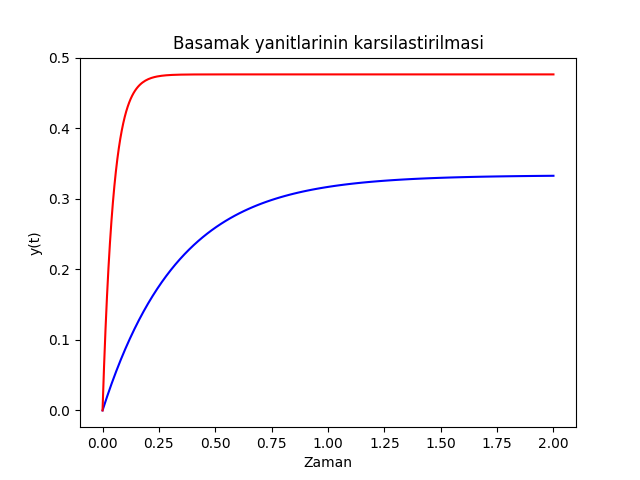
\includegraphics[width=0.65\textwidth]{response}
        \caption{Basamak yanıtlarının karşılaştırılması}
    \end{figure}